\documentclass[crop,tikz]{standalone}

\usepackage{pgfplots,siunitx}
\pgfplotsset{compat=1.17}
\tikzset{>=latex}

\pgfplotsset{
  every non boxed x axis/.append style={
    axis line style={-latex}
  },
  every non boxed y axis/.append style={
    axis line style={-latex}
  },
  inverted/.style = {
    every axis legend/.append style={
      draw=white,
      fill=hardblack,
      text=white
    }
  }
}

\begin{document}
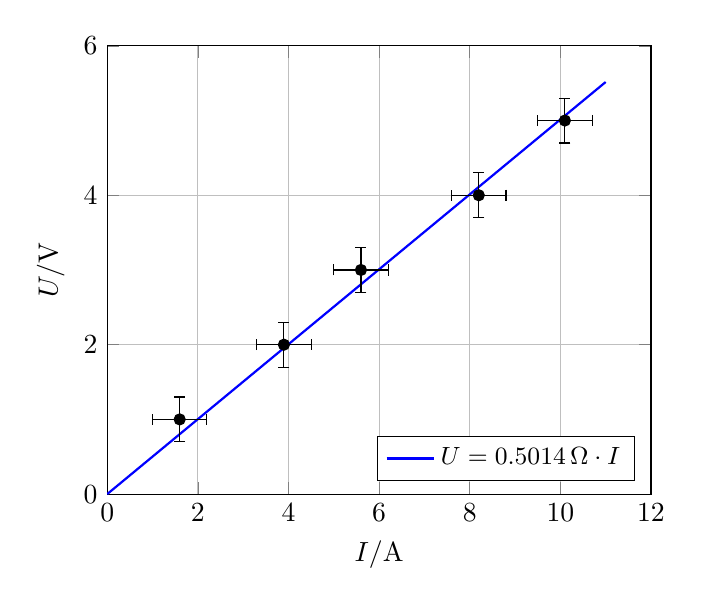
\begin{tikzpicture}
\begin{axis}[
  width={0.7\textwidth},
  height={0.6\textwidth},
  domain=0:11,
  xmin=0,xmax=12,
  ymin=0,ymax=6,
  xlabel={$I/\si{\A}$},
  ylabel={$U/\si{\V}$},
  grid,
  legend cell align = {left},
  legend style = {font=\small},
  legend pos = {south east},
  ]
  \addplot[blue, thick] { 0.5014*x };
  \addlegendentry{$U = \SI{0.5014}{\ohm}\cdot I$};
  \addplot[only marks, error bars/.cd, x dir=both, y dir=both, x explicit, y explicit] coordinates {
    ( 1.6, 1) +- (0.6, 0.3)
    ( 3.9, 2) +- (0.6, 0.3)
    ( 5.6, 3) +- (0.6, 0.3)
    ( 8.2, 4) +- (0.6, 0.3)
    (10.1, 5) +- (0.6, 0.3)
  };
\end{axis}
\end{tikzpicture}
\end{document}
